%!TEX root = ../thesis.tex
% ******************************* Thesis Appendix B ****************************

\chapter{Packaging considerations for high temperature}
\label{app:Packaging}

The temperature affects the printed circuit board in several manner which are decomposed into material intrinsic properties alteration and material-material interfaces phenomena. For tests and measurements, we should consider both the mechanical and the electrical properties of the IC and the of the test boards.

\section{Package}
The package of an integrated circuit is an interface to the environment surrounding the chip whose desirable properties are a low thermal resistance to prevent the heat to be trap inside the package degrading ever more the Silicon electrical performance. The target design is close to the operating region where the carrier density is getting as sparse as within an intrinsic silicon bloc.
Therefore, the heat should be evacuated as quickly as possible while the selected package is as close as possible to the final one for relevant measurements. In addition to that, test under high temperature gives enough energy for most redox chemical reactions in which oxidations of contact and metals are expected to occurs.

Exposed to the environment, the package is thus selected based on its thermal-resistance to dissipate heat, its electrical insulation, and its protection from oxidation among many.

In order to output high frequencies signal for debug purpose, parasitic are intended to be minimized. This consider both the wire-bonding and the pins.

For the sake of simplicity, Table~\ref{tbl:high-temp-package} compares the properties of traditional package (plastic and ceramic) with fully closed encapsulation. Indeed, as large area of METTP is not allowed by the process manufacturing to prevent antenna effect, large area of metal have slits exposing the silicon based dielectric to the light. Partially closed or open IC allows visual verification of wire-bonding at the cost of substrate ionization by the absorption of light being more likely as the temperature increase (\(E_g\) is decreasing and a band gap shift occurs with the temperature~\cite{Lautenschlager1985,Klenner1992} while the Fermi-Dirac distribution becomes wider).

\begin{table}[htp]
    \centering
    \caption{Packing comparison for high temperature circuits}
    \label{tbl:high-temp-package}
    \begin{tabular}{lcccc}
    \hline
    \textbf{Mechanical Properties}                                                                       & \textbf{\begin{tabular}[c]{@{}c@{}}Ceramic Package\\ CLCC68\end{tabular}} & \textbf{\begin{tabular}[c]{@{}c@{}}Plastic Package\\ PLCC68 (PPS)\end{tabular}} & \textbf{\begin{tabular}[c]{@{}c@{}}Glob Top\\ S7503\end{tabular}} & \textbf{\begin{tabular}[c]{@{}c@{}}Glob Top\\ 50300HT\end{tabular}} \\ \hline
    Young Modulus {[}GPa{]}                                                                              & 150 -- 190                                                                & 6 -- 11                                                                         & NC                                                                & NC                                                                  \\
    Vickers Hardness {[}GPa{]}                                                                           & 5.9 -- 9                                                                  & 5                                                                               & NC                                                                & NC                                                                  \\
    Viscosity {[}Pa.s @ 10 rpm{]}                                                                        & NC                                                                        & NC                                                                              & 80 -- 100                                                         & 120 -- 140                                                          \\
    Shore D                                                                                              & NC                                                                        & NC                                                                              & 85                                                                & 95                                                                  \\
    Water Absorption {[}\%{]}                                                                & 0                                                                         & 0.02                                                                            & 0.14                                                              & 0.4                                                                 \\
    \textbf{Thermal Properties}                                                                          &                                                                           &                                                                                 &                                                                   &                                                                     \\ \hline
    \begin{tabular}[c]{@{}l@{}}Coefficient of Thermal\\ Expansion {[}$\mu K^{-1}${]}\end{tabular}        & 9.6 -- 11.5                                                               & 33                                                                              & 193                                                               & 18                                                                  \\
    \begin{tabular}[c]{@{}l@{}}Thermal\\Conductivity {[}$W/mK${]}\end{tabular}                                                           & 2 -- 5                                                                    & 0.29                                                                            & 0.22                                                              & 0.63                                                                \\
    \begin{tabular}[c]{@{}l@{}}Glass Transition\\Temperature Tg {[}$\degree C${]}\end{tabular}          & \textgreater 175                                                          & 170                                                                             & 175                                                               & 165                                                                 \\
    \textbf{Electrical Properties}                                                                       &                                                                           &                                                                                 &                                                                   &                                                                     \\ \hline
    \begin{tabular}[c]{@{}l@{}}Dielectric Constant {[}$@25 \degree C${]}\\ and Loss tangent\end{tabular} & \begin{tabular}[c]{@{}c@{}}6.5 / 0.0003\\ @ 1 MHz\end{tabular}            & \begin{tabular}[c]{@{}c@{}}3.0 / 0.0001\\ @ 1 kHz\end{tabular}                  & \begin{tabular}[c]{@{}c@{}}3.1 / 0.0005\\ @ 1 kHz\end{tabular}    & \begin{tabular}[c]{@{}c@{}}3.2 / 0.0009\\ @ 1 kHz\end{tabular}      \\
    Volume Resistivity {[}$10^{14}${]}                                                                     & 0.01 -- 4                                                                 & 0.1 -- 10                                                                       & 1                                                                 & 3.3                                                                 \\ \hline
    \end{tabular}
    \end{table}

For high temperature integrated circuits, the most physically robust solution is a ceramic package with a caution on the dielectric constant value which has a large discrepancy with most PCB material. Therefore, the plastic package is thus the most appropriate for test temperature below 160\(\degree C\). Willing to test the IC at 175\(\degree C\), and a chip size of 1.3 mm x 1.3 mm while a CLCC68 package would be of 25.4 mm x 25.4 mm the inductance of a wire connected at a corner would be of 26 nH. a Glob Top solution is good compromise which allows a chip-on-board connection limiting the inductance to 7 nH.

Considering discrete buffers whose pin's capacitance are 20 pF, the capacitance of the PCB trace of 7 pF and a pad capacitance of the IC of 1.9 pF, the cut-off frequency is boosted from 180 MHz to 353 MHz in the worst case. From another point of view the sampling frequency of ADC being 20 MHz, the settling has 9 to 17 times the time constant of the line.

One precaution that have been overlooked in the design but have a deep impact on results is a protection for the Glob Top to reduce the sensitivity to air pressure variation. In order to use commercial on-the-shelves components on a motherboard, the tests over temperature are performed with a thermal stream 5000 from MPI\@. The hot air is blown on the area delimited by its thermal enclosure. The temperature increasing the glob top tends to be malleable and the air pressure on the wire bonding. To limit the impact a cover has been placed over the daughter-board to let the air surrounding the IC heating but preventing a direct blown air on the IC as depicted by \figurename~\ref{fig:thermalstream-air-protection}.

\begin{figure}[htp]
    \centering
    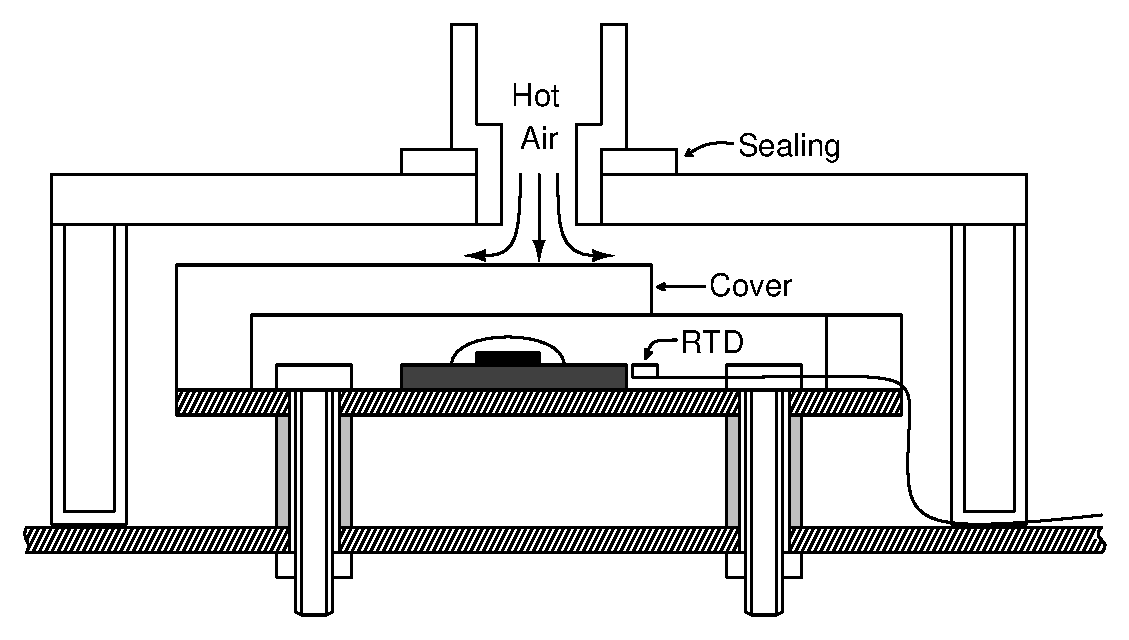
\includegraphics[width=0.8\textwidth]{Chapter5/Figs/PCB/thermal-stream-protection.ps}
    \caption{Protection against the blown air pressure variation inside the thermal enclosure of the thermal stream}
    \label{fig:thermalstream-air-protection}
\end{figure}

\section{Boards}
With regards to the PCB conception, the temperature increasing inflates the dielectric. The distance between metal layers changing, the dielectric constant is thus temperature dependent (at least from a geometrical point of view). Changes in z-axis CTE and dielectric constant as a function of temperature can significantly impact the impedance of strip transmission lines fabricated on that material while engendering a mechanical stress on soldering points and vias.

Because a material can undergo such a drastic change in CTE, it becomes mechanically and electrically unstable when operating above a defined temperature Tg, when the dielectric become soft and malleable. The PCB should always be maintained below that temperature except for short-duration processing steps, such as solder reflow.

% special case of the mother board
In the special case of the motherboard, more precisely at connections points with the daughter-board, pins from one connector are soldered to transmission lines. The pins connectors and transmission lines being in copper while the soldering is a dissimilar metal, an electromotive force appears at the junction coming from a thermal difference between each metal. Also called Seebeck effect, for a Copper-Lead-Tin Solder the coefficient of the electromotive force is 5 \(\mu V/\degree C \) which sufficient to generate an error of 500 \(\mu V\) for 100 \(\degree C\) between the two.

In order to perform the characterization of the ADC whose accuracy reaches 12-bits with an input excursion of \(\pm \) 1 V, the thermal difference shall not be higher than 24\(\degree C\). One way to cope with this effect is by waiting the establishment of the temperature before a characterization at a new temperature. In addition for sensitive nodes, differential signaling is recommended.

Even if differential signaling is done, a high speed signal over long trace is prone to power reflection. Therefore, both analog and digital traces, whose signal frequency is between 25 MHz and 100 MHz, have their impedance matched. A solution based on motherboard for signal generation and reshaping and a daughter-board with only the test chips under temperature is the most effective way to achieve the matching with test devices.

% buffers for digital to reduce large current from the ADC parts generating higher noise
On transmission lines for high speed digital, bidirectional buffers are added to keep the signal end-to-end clean. Digital buffers benefits are three fold: First, they adapt the signal from a 1.8 V voltage domain to a more traditional 3.3 V to 5 V of digital test device (LVDS IP usually consider a 3.3 V voltage domain). Second, splitting the signal path into several chunk, the impedance matching is easier to realize between the IC and the buffers. And as the digital lines of test devices have an impedance of 150 \(\Omega \) to 300 \(\Omega \), the matching not being perfect from the test devices to the buffers will only have low-reflection capacitance. During the conception the maximum allowed power reflected is 10 \% which corresponds to a maximum VSWR (voltage standing wave ratio) equal to 1.22 which is in nutshell an error due to mismatch of 30 \(\Omega \). Third without them, the digital pads of the IC should provide a large current to charge and pump the capacitance of test devices. The large transient current generates a large noise whose decoupling from the analog core is more difficult. By the addition of buffers, the capacitive load is reduced and the generated noise is decreased.

% capacitors and decoupling
To enhance the performance, it is critical to place the reservoir capacitor close to the ADC’s sensitive inputs. Among the most sensitive ones are reference input pins, input voltages, and power supplies. While the input pins are high speed signals, the impedance matching is supposed to be sufficient. For practical reason small capacitors are needed to filter out possible coupling noise. 

\begin{figure}[htp]
    \centering
    \begin{subfigure}[c]{0.8\textwidth}
        \includegraphics[width=\textwidth]{Chapter5/Figs/PCB/decoupling_cap_reference.ps}
    \end{subfigure}
    \begin{subfigure}[c]{0.8\textwidth}
        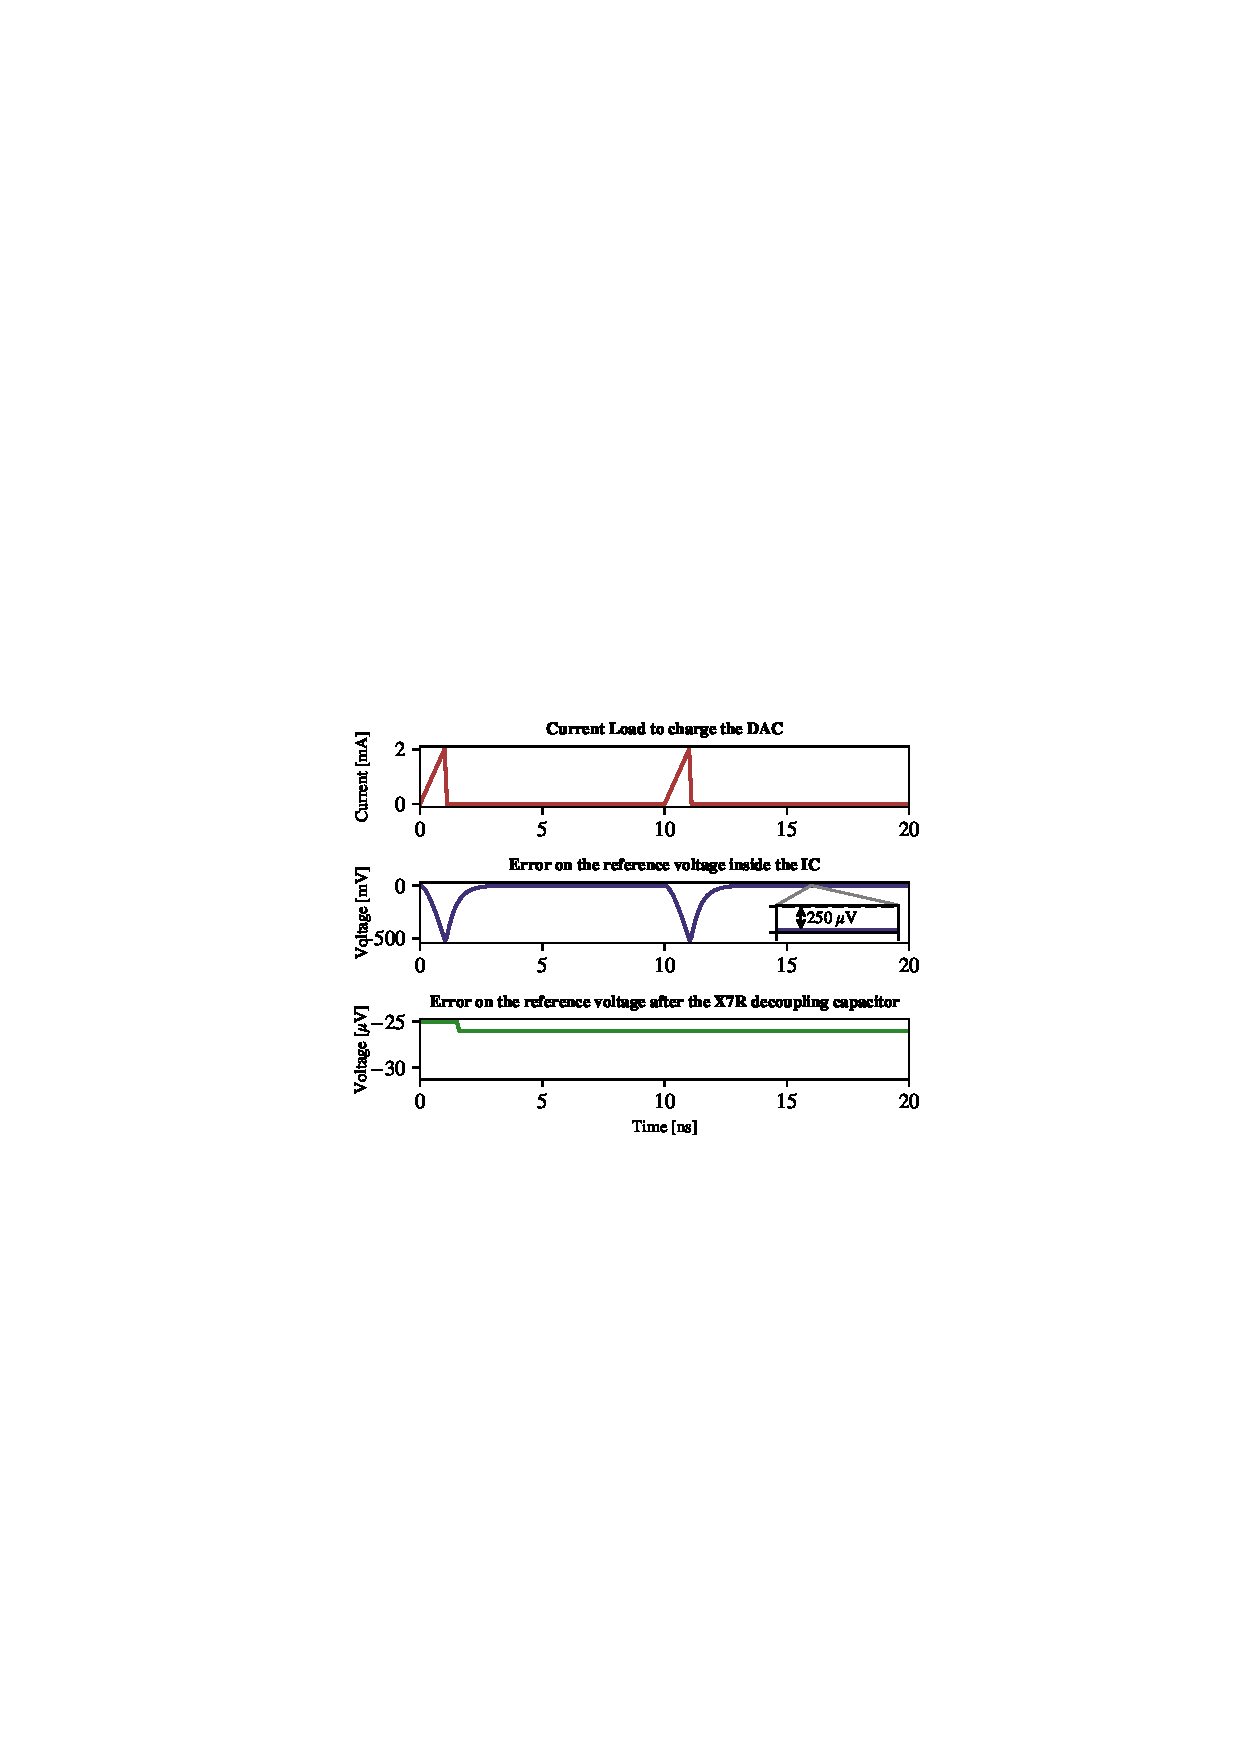
\includegraphics[width=\textwidth]{Chapter5/Figs/PCB/decap-reference-sar.pdf}
    \end{subfigure}
    \caption{Decoupling strategy to reduce recovery time and the settling error on references}
    \label{fig:decoupling-strategy}
\end{figure}

But for DC signals such references and power supplies, the filtering network depends on the load and the current profile. For instance, on the SAR sub-ADC the power supply shall be feed large transient current the comparator while the reference drops only while the reference is connected to the DAC\@. The capacitor acts as a charge reservoir with charge pumped by the load and re-filled at a rate depending from the resistivity of the path for re-filling, \figurename~\ref{fig:decoupling-strategy}. To decrease the minimum time to recover, decoupling capacitors have been split into one inside the IC chip and several outside. To prevent oscillations the ESR of decoupling capacitors is minimized by using multiple vias to a ground plane and using wide traces to connect them. Ceramic capacitors with X7R dielectric are a good choice close to IC where the temperature is the highest (175 \(\degree C\)). Then outside at ambient temperature a large 470 \(\mu F\) electrolytic capacitor filter the voltage provided by the power supply source, such as an Hameg HMP 4040. 

For the sake of clarity others phenomena such as power derating, voltage derating, temperature drift,\ldots are considered but not detailed.
